\chapter{Molecular Line Survey}

\section{Previous Work}

There have been two main types of surveys for searching for CO emitters in the universe, targeted and blind surveys. In targeted surveys, targets are chosen based on some type of preselection, such as star formation rate, mass, or some other parameter [CITE], and are looked at specifically to see what CO emissions can be found in that galaxy or galaxies. While this gives a lot of useful information on the role gas plays in these galaxies [MORE SPECIFIC], the preselection process means that there could be a bias in our knowledge of CO. Because most preselection is based on star formation rate and mass, or brightness in some other wavelength, these surveys could miss out on dark, gas-rich galaxies that are hard to see otherwise, giving us an incomplete picture of the variety of galaxies with gas and CO emission in the universe. 

Blind surveys are the opposite of targeted surveys. Instead of choosing the targets and looking at them specifically, blind surveys choose an area of the sky and search for any CO emissions within that cosmic volume, allowing for any emissions above the sensitivity limit of the survey to be found. This allows for a sort of census of all the gas within a cosmic volume [CITE]. 

Previous blind surveys include the COLDz survey [EXPAND ON THAT] in the GOODS-North region, the PdBI survey [EXPAND], as well as the first two surveys in the ASPECS program, ASPECS Pilot and ASPECS Large Program. 

The ASPECS Pilot and Large Programs both looked at regions in the Hubble Ultra Deep Field, with Wide ASPECS being the third survey in the sequence. The Pilot program looked incredibly deeply in the 1.2mm and 3mm bands at a small, one arcsecond region of the Hubble eXtremely Deep Field (XDF). The spectral coverage of the Pilot meant that it could detect CO transitions almost continuously from z = 0 to z = 8, as well as CII emissions from z = 6 to z = 8 \cite{walter2016alma}. This allowed for the characterization of CO emitters all the way to a z = 8, as well as given constraints on the knee of the CO luminosity function [CITE]. 

The Large Program looked wider, but shallower, covering a roughly five square arcminute area of the Hubble Ultra Deep Field (HUDF) surrounding the ASPECS Pilot region. It was a 150 hour molecular deep field taken at 1.2mm and 3mm \cite{decarli2019alma}.  The greater volume probed by the Large Program allowed for constraining the density of gas in the Universe, as well as better constraints on the CO luminosity function. The survey blindy revealed the molecular gas content in normal, star-forming main-sequence galaxies \cite{decarli2019alma}. 

\section{This survey}

\begin{figure}[tbp]
\centering 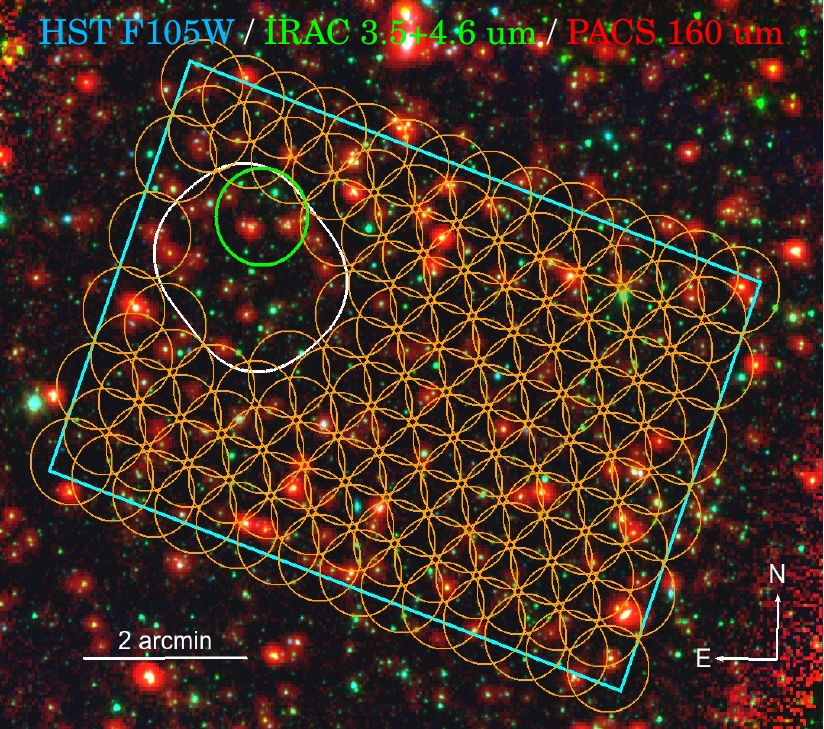
\includegraphics[width=120mm]{Wide_ASPECS_Coverage.png}
\caption{Spatial coverage of ASPECS Pilot (Green), Large Program (White), and Wide (Yellow) showing each of the individual pointings. The area covered by the Pilot is $~$1 arcmin$^2$, by the Large Program $~$5 arcmin$^2$, and by Wide ASPECS, $~$52.5 armin$^2$. The cyan box is the extent of the CANDELS-South region, showing where a wealth of ancillary data has been collected in over 30 wavelengths [CITE].}
\label{fig:ASPECS_Coverage}
\end{figure}

\begin{figure}[tbp]
\centering
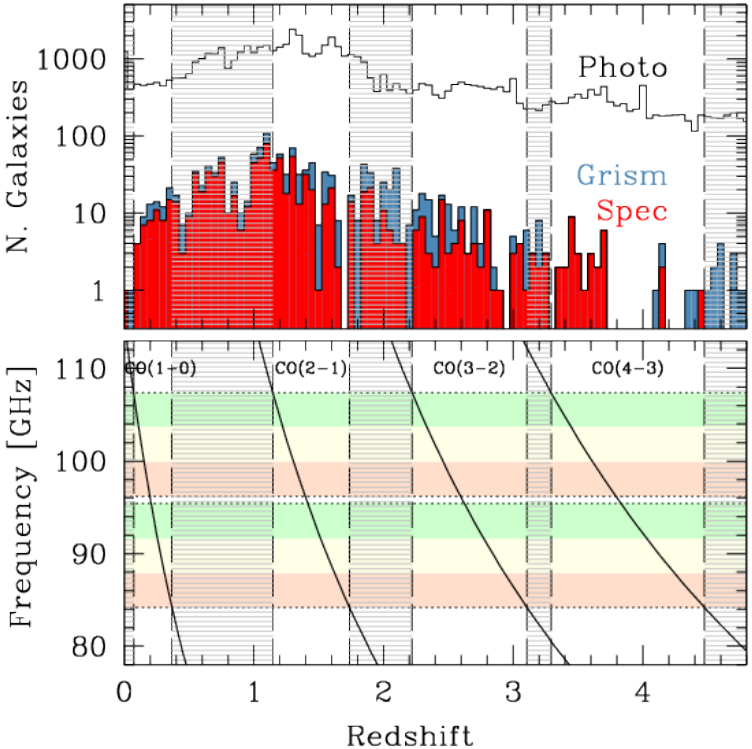
\includegraphics[width=120mm]{Wide_ASPECS_Freq.png}
\caption{Spectral and redshift coverage of Wide ASPECS. Wide ASPECS is designed to detect CO line transitions at z$<$0.4, 1.1 $<$ z $<$ 1.8, and 2.2 $<$ z $<$ 4.4. [CITE OR CHANGE PLOT]}
\label{fig:ASPECS_Freq}
\end{figure}


The Wide ASPECS survey builds upon the Pilot and Large Program, going much wider, but also shallower. This means that Wide ASPECS cannot capture as dim CO emitters, but because of the much larger cosmic volume looked at, it can find rarer, but very bright CO emitters that did not happen to fall within the Large Program and Pilot survey bounds [CITE/EXPAND]. 
The data for this survey was observed in ALMA Cycle SOMETHING and was done in [SURVEY DESCRIPTION]. This raw data was processed with CASA (). This resulted in 6 data cubes, one for each frequency setting. 

\subsection{Ancillary Data}

In addition to each of those datacubes, there is a lot of ancillary data available as the GOODS-South region is one of the most studied regions of the sky. This data has been collected through combining multiple other catalogs, first described in [LIST OF CATALOGS], comprising over 30 wavelength bands for over 63000 galaxies in and around the footprint of Wide ASPECS. 26000 galaxies lie within the footprint of Wide ASPECS, of which ~4000 have spectroscopic redshifts, and 22000 have photometric redshifts. 

The majority of the ancillary data comes from the Hubble Space Telescope (HST) Cosmic Assembly Near-infrared Deep Extragalactic Legacy Survey (CANDELS; Grogin et al. 2011; Koekemoer et al. 2011). Most of the photometric data comes from Skelton et al (2014), which additionally includes ground-based optical and NIR photometry from Nonino et al. (2009), Hildebrandt et al. (2006), Erben et al. (2005), Cardamone et al. (2010), Wuyts et al. (2008), Retzlaff et al. (2010), Hsieh et al. (2012), as well as Spitzer IRAC 3.6um, 4.5um, 5.8um, and 8.0um photometry from Dickinson et al. (2003), Elbaz et al. (2011), and Ashby et al. (2013). There is also data from the Spitzer MIPS 24um photometric information from Whitaker et al. (2014), and ALMA 1.1mm data from Franco et al. (2018). Additional far-infrared data from Herschel PACS at 100 um and 160 um from Elbaz et al. (2011). Data from the MUSE Hubble Ultra Deep Survey (Bacon et al. 2017) was also included, being used for spectroscopic redshifts (Inami et al. 2017), other catalogs used for spectroscopic information include Le Fevre et al. (2005), Coe et al. (2006), \cite{skelton20143d}, and Morris et al. (2015). Hubble grism spectroscopy was taken from the 3D-HST survey \cite{momcheva20163d}.  All these catalogs were merged into a single catalog through matching sources within 0.5 arcseconds for the photometry, and 1.0 arcseconds for the spectroscopic data. Finally, these matches were then cross-matched with morphological parameters from ven der Wel et al. (2012). Within the Wide ASPECS footprint, $>$ 26000 galaxies are present, of which [INSERT HOW MANY SPECTROSCOPIC HOW MANY PHOTOMETRIC].

[GO THROUGH THE GALAXY TRIMMER, KEEP THE LINE IF THE POINT PASSES INSPECTION, THEN DO THE CALCULATION FOR PHOTO AND SPECTROSCOPIC, SAVE OUT CATALOG TO THEN RERUN THE STUFF ON]

\subsubsection{MAGPHYS}

One program that does this is MAGPHYS \cite{da2008simple, da2015alma}. MAGPHYS uses precomputed models to fit to the SED and create likelihoods on the different parameters that makes up an SED. This allows us to estimate the mass, star formation rate, dust temperature, etc. using as the input the SED and the redshift of the galaxy. In the SED fitting, different components of the galaxy contributes to different wavelengths. Young stars are bright in the UV and visible spectrum, so many young stars pushes a galaxy's SED more into the UV end of the spectrum. On the other hand, gas and dust absorbs the light from stars within the galaxy and re-irradiates that light as infrared, making a galaxy with lots of gas be redder and dimmer than one without. The SED takes all of this into account, and MAGPHYS outputs a likelihood distribution for the different parameters, as well as the best-fit total SED for a given galaxy. An extension of MAGPHYS, the MAGPHYS high-z extension \cite{da2015alma}, which takes into account more of the [INCLUDE MORE ON HIGH Z DIFFERENCES] was used for the SED fitting in this report. 

An example output from MAGPHYS is shown in Fig. \ref{fig:MAGPHYS_Example}, showing the model, the likelihood values for various physical properties of the galaxy, and the data points used to compute the SED in red.

\begin{figure}[tbp]
\centering 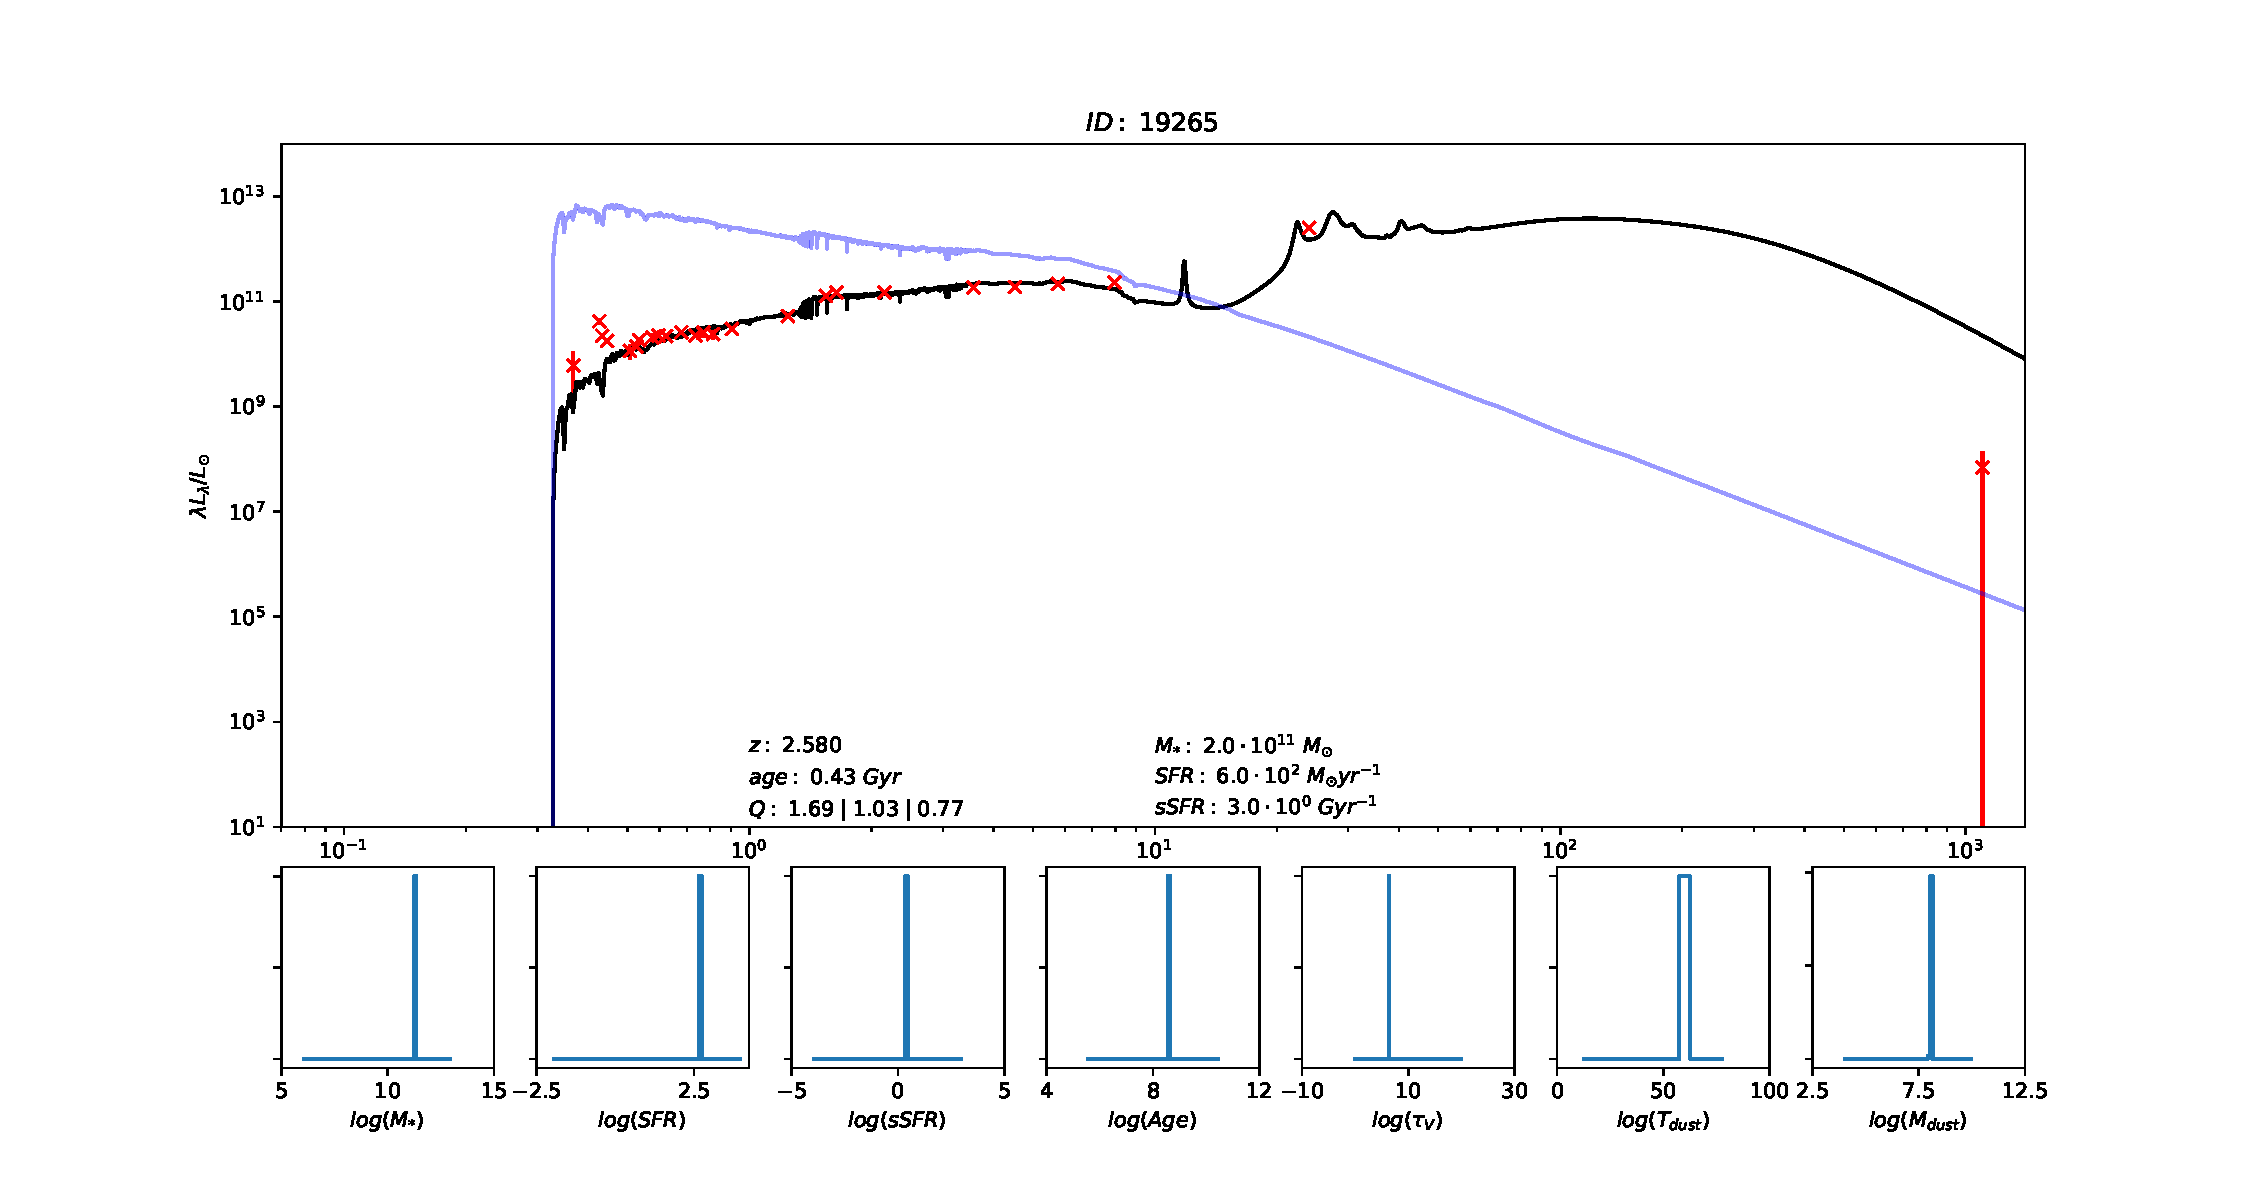
\includegraphics[width=120mm]{19265.pdf}
\caption{Example MAGPHYS Output, from the most massive matched galaxy. The blue line is the spectrum of the galaxy without attenuation. The black line is the model used by MAGPHYS. The red dots are the data points. The bottom row of graphs show the probability distribution for various physical properties.}
\label{fig:MAGPHYS_Example}
\end{figure}

\section{Method}

As an overview, the method for finding lines, computing the fidelity, cross-matching, and determining matches is the same process as used in the other ASPECS surveys \cite{walter2016alma, decarli2019alma}. The galaxies' properties were estimated by using MAGPHYS to fit their SEDs. [MAKE SMOOTHER]

\subsection{Line Search and Fidelity}

To find possible CO emitters, a search for CO lines is done by the findclumps algorithm first described in \cite{walter2016alma} [AND NEW LINE SEARCH ONE]. This code searches along the spectral axis with different kernel widths in order to maximize the sensitivity to signal associated with line candidates of different intrinsic widths. The data cubes are searched for lines at any spatial position and spectral coordinate, without any prior based on data from other wavelengths. This is done to minimize any bias in the selection function. findclumps returns a list of potential line candidates that then have duplicates removed, which is done by grouping line candidates based on their spatial and spectral position in the cube from each group, only storing the candidate with the highest S/N. This results in 11941 candidates at S/N$>$5.0, 1096 at S/N$>$5.5, 78 at S/N$>$6.0, and 6 at S/N$>$6.5. 

To get a sense of how many of these line candidates are false positives, the fidelity of the lines are then computed. To obtain the fidelity, a line search on the negative data cubes is performed. The negative cubes are obtained by multiplying all the values in each data cube by -1, and rerunning the line search. This catalog of negative lines is then used to compute the fidelity. The fidelity of a line at a given S/N and line width, $\Delta v$, is defined as 

$$ fideltiy(S/N, \Delta v) = 1 - \frac{N_{neg}(S/N, \Delta v)}{N_{pos}(S/N, \Delta v)} $$ [CITE].

The fidelity of the different line widths are shown in Fig. \ref{fig:Fid_map}. As can be seen, the fidelity of the lines is larger for wider line widths. For this report, there were 16 lines at a fidelity $>$0.8, 20 at $>$0.7, 35 $>$ 0.6, 52 $>$ 0.5, and 69 $>$ 0.4. The fidelity cut used for the rest of this analysis is set at 0.6, where every given line has a 60\% chance of being a real line, and leaving us with 35 line candidates. [INCLUDE TABLE OF FIDELITY, S/N PER WIDTH, NUMBER OF LINES?]

\begin{figure}[tbp]
\centering 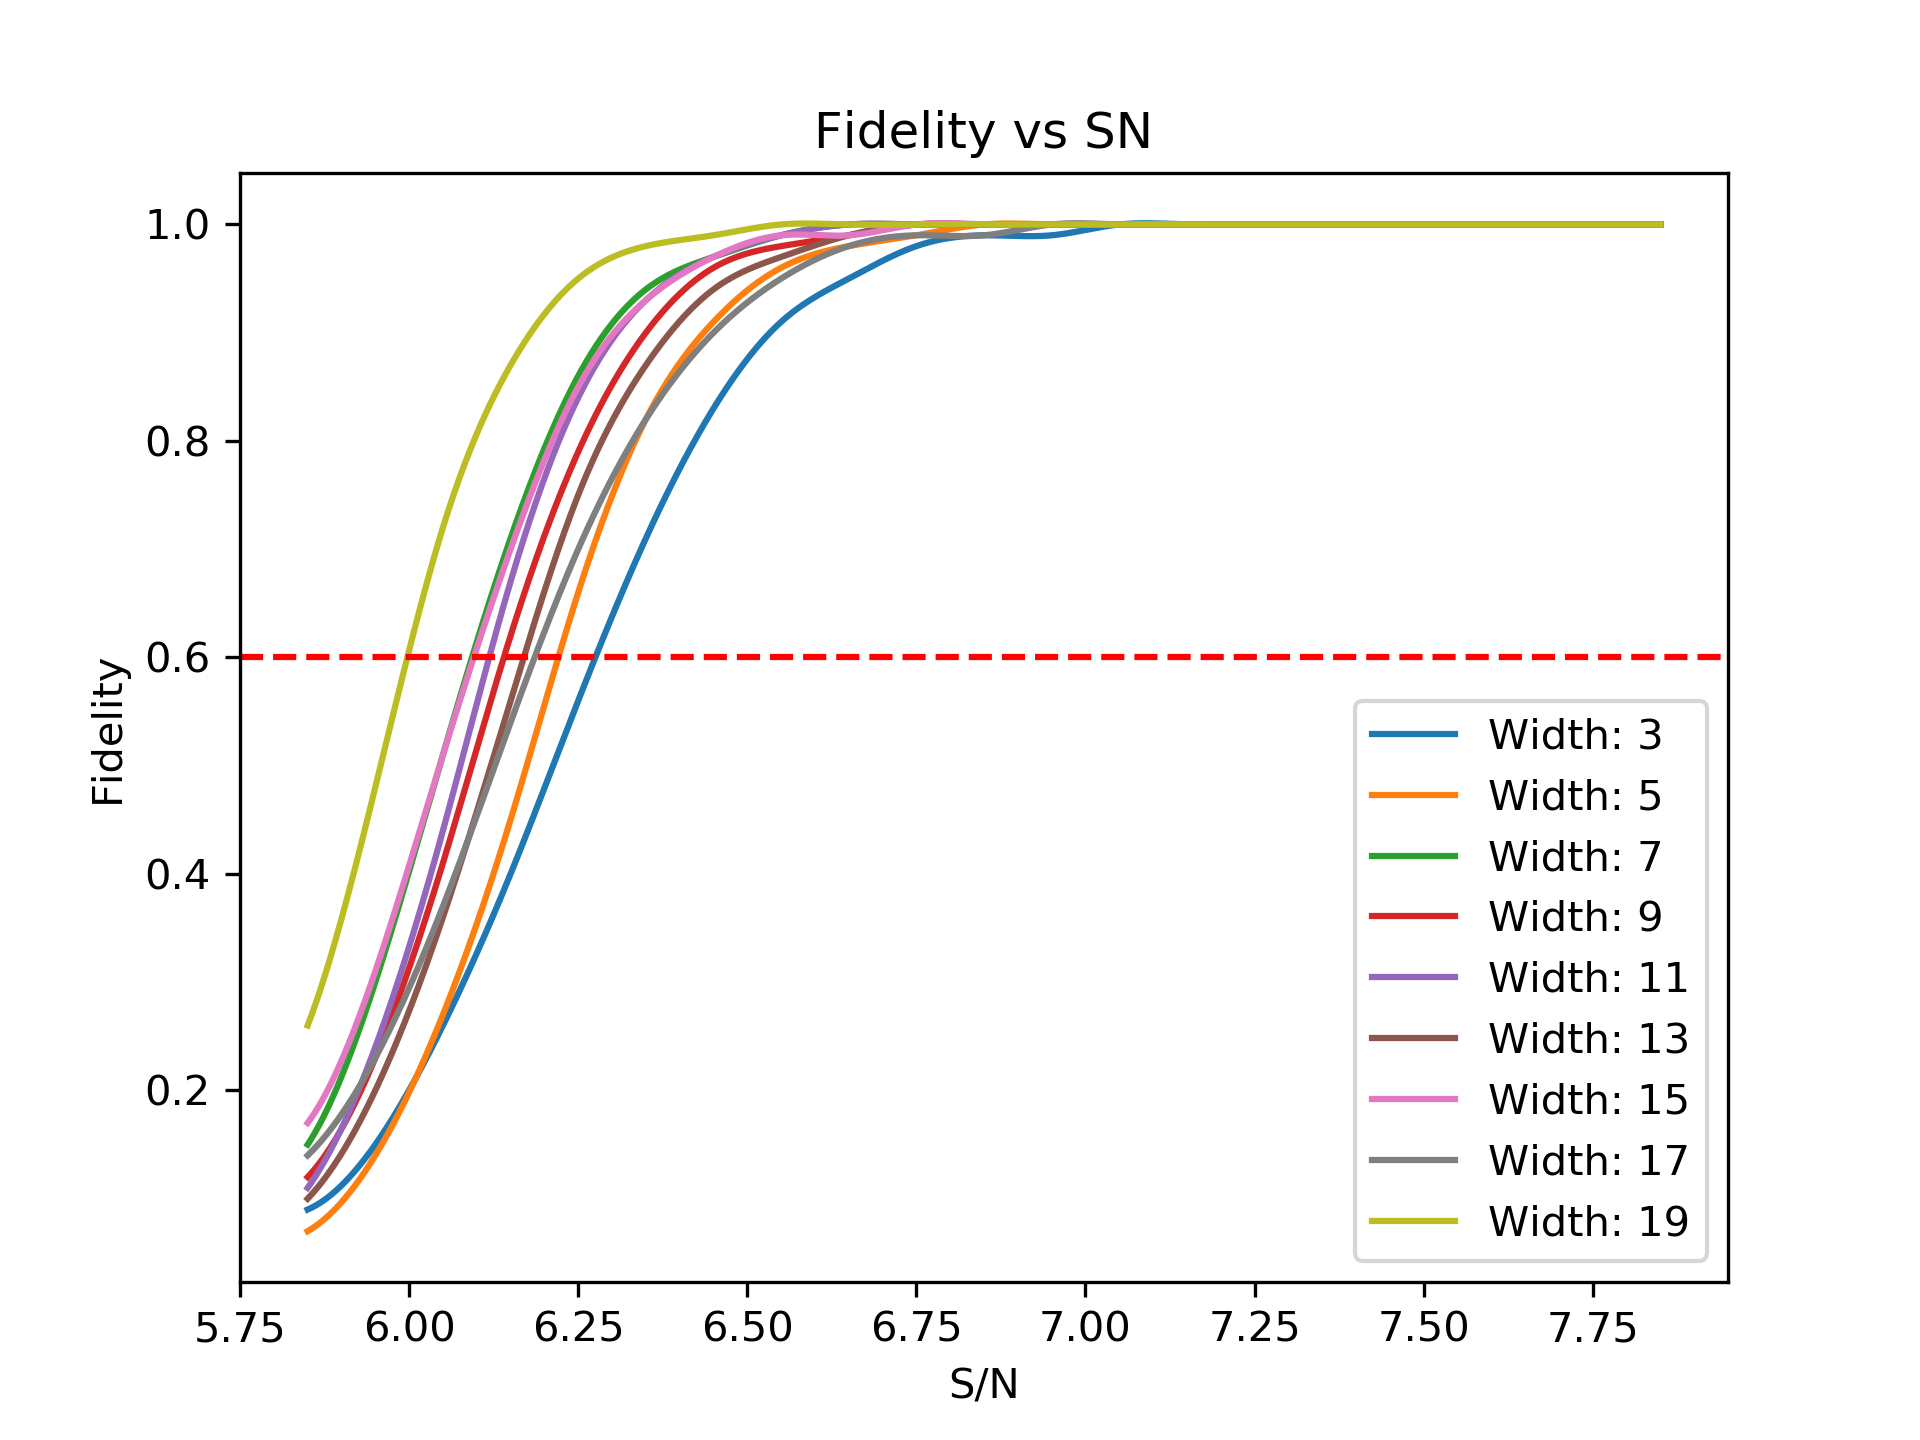
\includegraphics[width=120mm]{Fidelity_map.png}
\caption{Fidelity vs S/N for the different widths used by findclumps. The red line shows the fidelity = 0.6 cutoff used for the analysis in this report.}
\label{fig:Fid_map}
\end{figure}

\subsection{Cross-matching and redshift determination}

Once the lines and been found, and the fidelity computed, the next step is to cross-match the CO lines to already known galaxies within the Wide ASPECS footprint. To do this, the spatial location of the line candidates were matched to galaxies that were within one arcsecond of the line candidate's location. If a line matched to more than a single galaxy, then the following steps are performed to differentiate which galaxy the line should be matched to. The first step is to calculate the CO transition for the line assuming the line is matched to each of the galaxies. Once that is determined, the difference in redshift between the CO redshift and the galaxy's redshift, the $\delta z$, is calculated. The matched galaxy that gives the smallest $|\delta z|$ is then saved as the matched galaxy for that line candidate. 

To determine the redshift of the line candidates a few different steps were taken. As there are multiple CO transitions contained within frequency range for Wide ASPECS, a few different approaches are used to attempt to estimate the correct redshift. The first step is to attempt to match a line to one of the galaxies in the catalog. If there is a match in the catalog, then the available redshift of the matched galaxy is used for the redshift of the CO line. If the redshift of the matched galaxy is within the limits that Wide ASPECS can detect. The redshift determinations were only kept if the CO redshift was in very good agreement with spectroscopic redshifts ($|\delta z| < 0.01$) or ($|\delta z| < 0.3$) for photometric redshifts. [WHY DO THIS? CITE BOOGARD LP Paper]

If there is not a match to a galaxy in the catalog, or if the galaxy's redshift is incompatible with the CO line identification, then the line identification is performed by a bootstrap method, where the probability of a line candidate being one of CO(1-0), CO(2-1), CO(3-2), or CO(4-3) is proportional to the volume of the universe sampled in each of those transitions. [CITE WALTER? DECARLI AT LEAST] 

\section{Results}

The mass versus star formation rate is shown for the general galactic population and the ASPECS sources in Fig. \ref{fig:Cross_match}. For comparison, the Schreiber et al. 2015 \cite{schreiber2015herschel} and Walter et al. 2014 [CITE] main sequences are plotted as well. As can be seen, two of the matched galaxies are above the main sequence and are massive, star-forming galaxies that are the expected type of galaxies for this survey to match to. The other galaxy is much less massive than expected.

\begin{figure}[tbp]
\centering 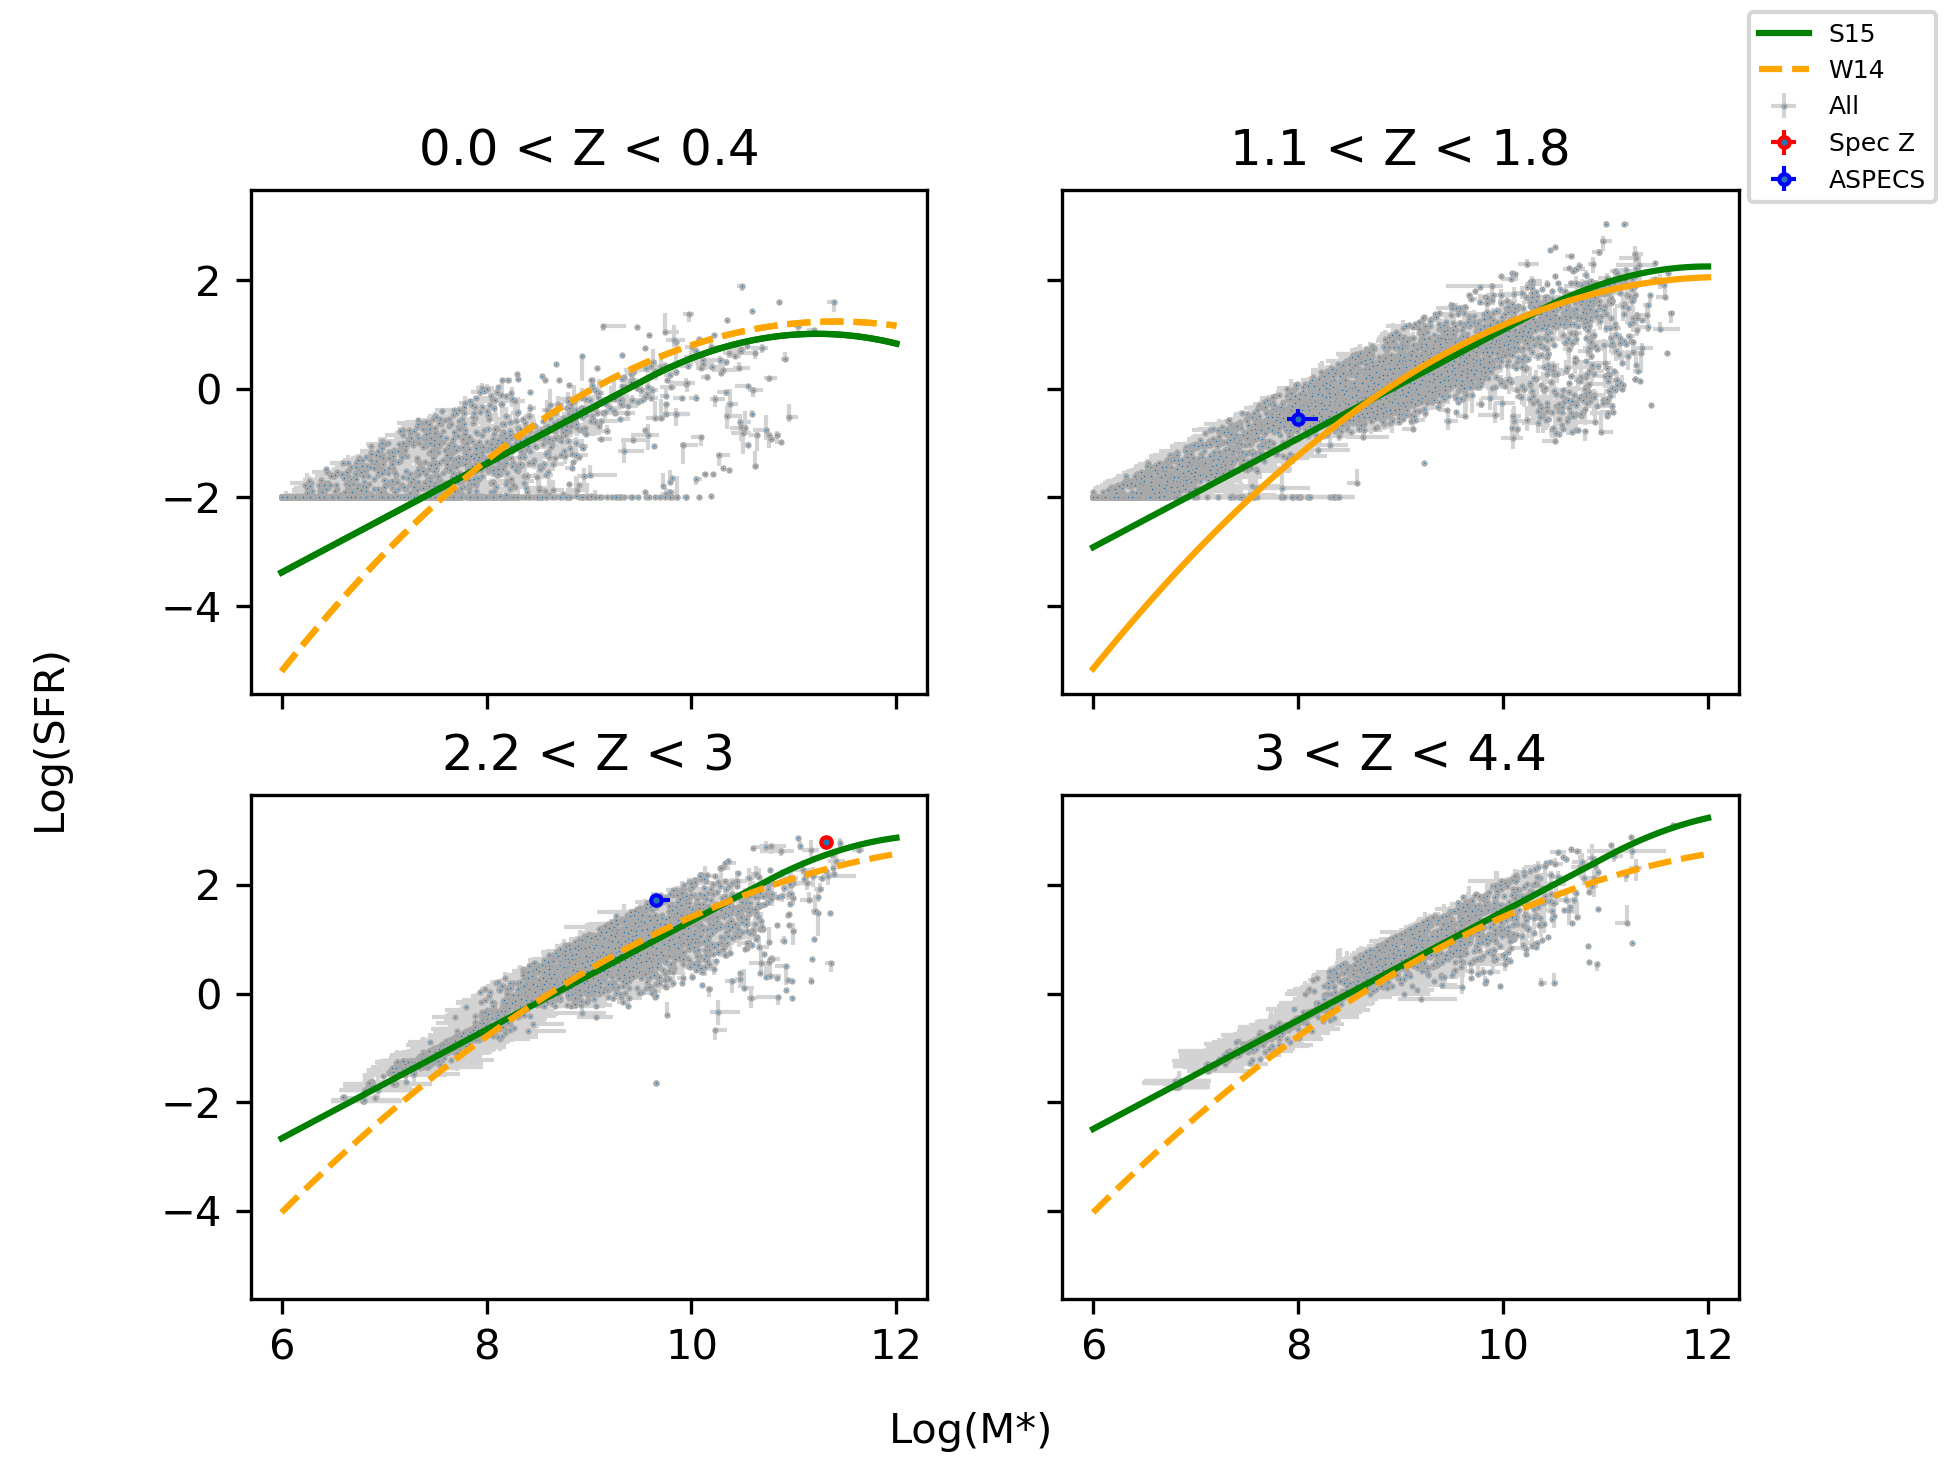
\includegraphics[width=120mm]{Mstar_vs_SFR_all_closest_sep_1_0_sn_fid_60.png}
\caption{Mass vs Star Formation Rate for the matched galaxies. Red points are matched galaxies with spectroscopic redshifts, while blue points are matched galaxies with photometric redshifts. Grey points are all the galaxies in the catalog. The green lines are the Schechter 2015 galaxy main sequence fit. The yellow line is from Walter et al. 2014's galactic main sequence fit, where the solid line means it is computed within the range mentioned in the paper, while dotted means that the values are extrapolated from the paper to higher, or lower, redshifts. Two of the three matches are on the upper edge of the main sequence, while the third match has a much lower mass and star formation rate than expected for this survey.}
\label{fig:Cross_match}
\end{figure}

\subsection{Catalog}

The final catalog of CO line emitters is shown in Table \ref{table:Catalog}. 

[INCLUDE IDs FOR THE MATCHED ONES?, SORT BASED ON S/N, MAKE LOOK LIKE OTHER TABLES?, INCLUDE ALL 35 LINES, EVEN THOSE WITHOUT LINE IDENTIFICATIONS]

\begin{table}
\centering
\caption{RA and DEC are in the J2000 system. $v_{CO}$ is in GHz. CO trans. is the estimated CO transition. $z_{catalog}$ is the redshift in the catalog. }
\begin{tabular}{ccccccccc}
RA & DEC & $v_{CO}$ & CO trans. & $z_{catalog}$ & $z_{CO} $ & $\Delta$Z & $\Delta$V & S/N \\
53.11881 & -27.78291 & 104.501 & 3-2 & 2.39 & 2.309 & 0.08 & 7338.53 & 6.43 \\
53.14886 & -27.82118 & 96.701 & 3-2 & 2.582 & 2.576 & 0.01 & 503.01 & 7.31 \\
53.16066 & -27.76629 & 86.677 & 2-1 & 1.423 & 1.66 & -0.24 & -26710.83 & 6.6 \\
53.13447 & -27.74976 & 102.719 & 3-2 & -- & 2.366 & -- & -- & 6.49 \\
53.11066 & -27.82727 & 85.654 & 3-2 & -- & 3.037 & -- & -- & 6.45 \\
53.06316 & -27.82356 & 84.623 & 3-2 & -- & 3.086 & -- & -- & 6.15 \\
53.07696 & -27.8251 & 90.891 & 2-1 & -- & 1.536 & -- & -- & 6.42 \\
53.09146 & -27.8497 & 106.235 & 3-2 & -- & 2.255 & -- & -- & 6.27 \\
53.1179 & -27.8184 & 92.876 & 2-1 & -- & 1.482 & -- & -- & 6.21 \\
53.11182 & -27.82032 & 99.522 & 4-3 & -- & 3.633 & -- & -- & 6.19 \\
53.09788 & -27.76003 & 90.618 & 3-2 & -- & 2.816 & -- & -- & 6.13 \\
53.14828 & -27.84444 & 87.302 & 3-2 & -- & 2.961 & -- & -- & 6.1 \\
53.07796 & -27.80182 & 98.725 & 4-3 & -- & 3.67 & -- & -- & 6.36 \\
53.07121 & -27.82724 & 88.954 & 3-2 & -- & 2.887 & -- & -- & 6.17 \\
\end{tabular}
\end{table}\label{table:Catalog}

[DISCUSS TABLE MORE]


\section{Discussion}

There are significantly less matches than was expected. Only $~$10\% percent of the lines match to galaxies. Of those that do, only two matched to the kind of galaxies that were expected, which are the most massive, most star forming galaxies in the field. 

Possible explanations include issues with MAGPHYS' fitting of the galaxies in the catalog, as many of the galaxies seem poorly constrained. 